\chapter{Background}
\label{cha:Background}
\quad Machine Learning (ML) is a field of inquiry devoted to understanding and building methods that learn, methods that leverage data to improve performance on certain set of tasks. It deals with the creation and training of models that can learn from data. An ML model is a file produced from a training procedure built with specific characteristics. The base ML model is composed of neurons grouped inside layers, connected in series (as pictured in figure \ref{base_neural_network}). The layers can be divided into the input layer, hidden layer, and output layer. The first layer, which is the input one, has the task of taking an input array (usually a matrix) where each neuron in the layer represents a value of the input. The following steps are hidden layers that take a certain number of input and convolute them with values called weights. Upcoming there are the output layers which depending on the model can represent different types of information such as bounding box or percentages representing classification.   

\begin{figure}[!ht]
\centerline{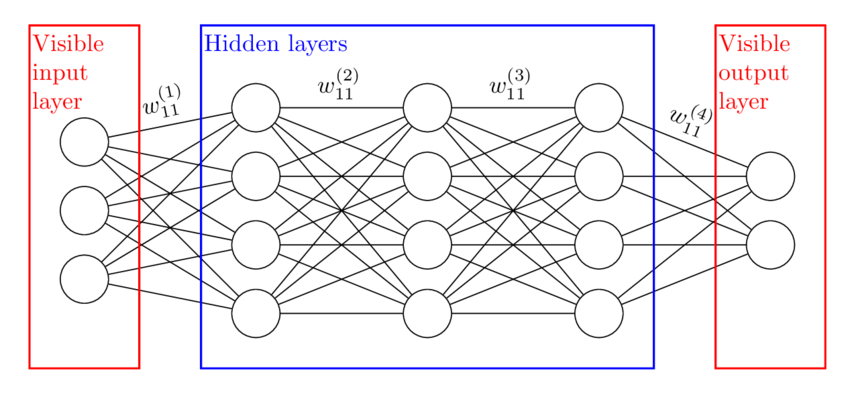
\psfig{file=Images/An-example-of-a-deep-learning-neural-network-with-3-hidden-layers.png,width=0.8\textwidth}}
\caption{Example of layers inside a base ML model \cite{Quantum_machine_learning}}
\label{base_neural_network}
\end{figure}

\section{Convolutional Neural Network}
\label{sec:context}
\quad The network taken into account in this paper is a convolution model, a Supervised Deep Learning model used for Computer Vision. The base operator is the neuron that grasps inputs and throughout operations gives an output. The differences between a NN and a CNN are the convolutional layers used to apply the convolution operation on images and thee pooling layers used to downsize the images through each layer (figure \ref{cnn_neural_network}). These two together encompass feature selection (extraction). Weights are also applied differently than the base model because they are allocated into kernels. Each kernel is used to filter a smaller area of the matrix given by the previous layer. The result is called a feature map. At each iteration, the kernel computes the convolution in a given area and then it slides off by a  value called stride. The last set of layers is the Fully Connected Layers (FC layer) which are a combination of Affine function and Non-linear functions such as Sigmoid, TanH, and ReLu. A Fully Connected Layer takes input from a flattened layer, a one-dimensional layer (1D layer). The data coming from the flattened layer is passed first to the Affine function and then to the non-linear one. In the end, is the softmax function that adds up the values to their corresponding final result and outputs the percentage of each class.

\begin{figure}[!ht]
\centerline{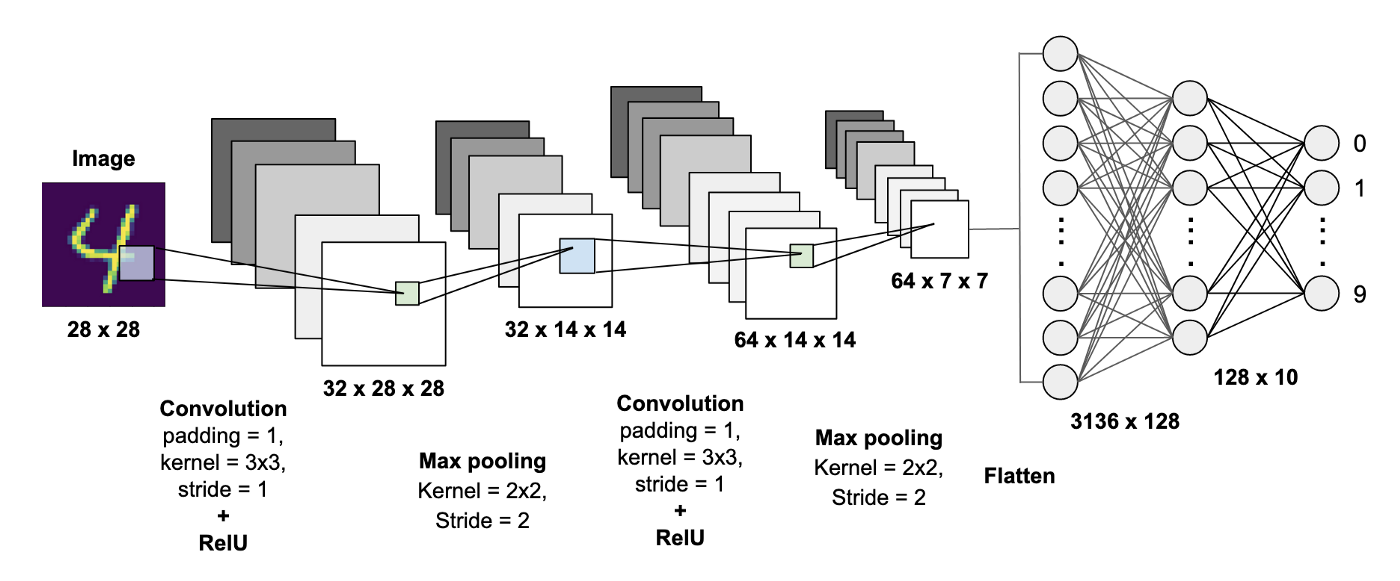
\psfig{file=Images/An-example-of-convolution-neural-network.png,width=0.8\textwidth}}
\setcaptioncitation{https://miro.medium.com/max/1400/1*SGPGG7oeSvVlV5sOSQ2iZw.png}
\caption{Example of layers inside a CNN model}
\label{cnn_neural_network}
\end{figure}

\section{Continual on-line learning}
\label{sec:CL}
\quad Machine learning applications base their functionality on the use of trained models for the elaboration of Data. One of the main aspects of ML applications is their capability to perform only inference over input samples. These systems are implemented with the only purpose of performing inference which is a sufficient requirement for typical applications. However, the usage of ML models capable of only predictions on known classes is not enough in some scenarios.
Currently, the scenario in which an ML model is placed, is a dynamic environment that is exposed to continuous evolution and changes, this leads to Data becoming obsolete quickly. Since TinyML applications are usually deployed for an extended period, scenarios like these one are common. To overcome the matter in question it is necessary to implement agents that render models self-adjustable and autonomous: a branch of ML that works on this topic is Continual Learning (CL). CL refers to the ability of a system to learn over time from a continuous stream of data without having to revisit previously encountered training samples. CL add the possibility to take a pre-trained model and update its parameters to adapt them to new Data. The Continual Learning approach focuses on the implementation of autonomous agents that control data streams and real-time ML training, with a particular focus on the implementation of fine-tuning strategies for the avoidance of out-of-date models. Continual learning is an already known topic in the field of research about machine learning. Lately it is gaining attention thanks to recent works in the sector of TinyML. The applications of CL on microcontrollers and specifically on IoT devices lead to better-performing systems with many benefits.

\begin{figure}[!ht]
\centerline{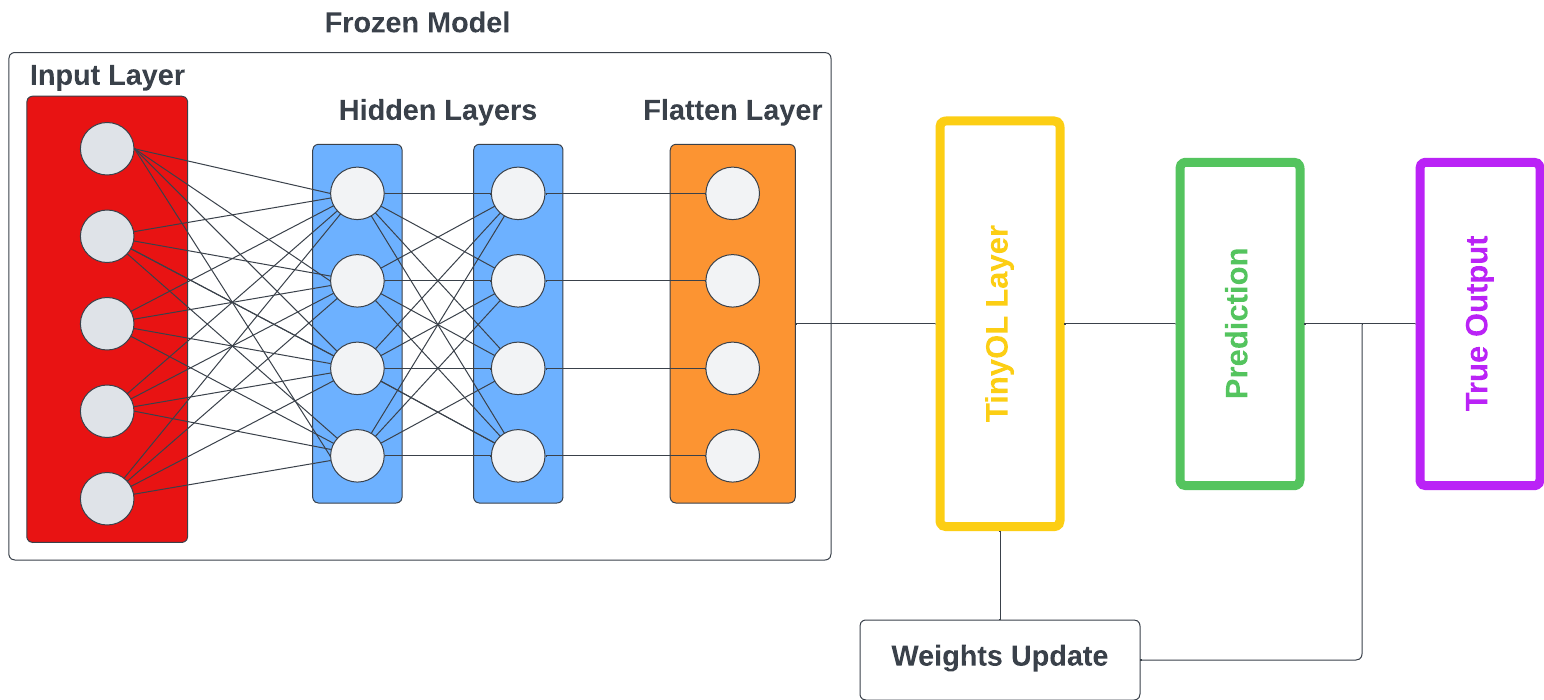
\psfig{file=Images/TinyOL_Machine_learning_network_model.png,width=0.9\textwidth}}
\caption{TinyOL workflow}
\label{OL_network}
\end{figure}

\section{Hardware}
\label{cha:hwardware}
\quad This work employs the MAX78000 \cite{Max78000}, a new breed of AI microcontroller built to enable neural networks to execute at ultra-low power and live at the edge of IoT. It has a feature that makes it stand out among the others: the hardware-based convolutional neural network (CNN) accelerator that enables battery-powered applications to execute AI inferences while spending only microjoules of energy. The accelerator is a perfect solution for TinyML applications thanks to its low energy consumption and the capabilities of running inferences in a short time. 

\begin{figure}[!ht]
\centerline{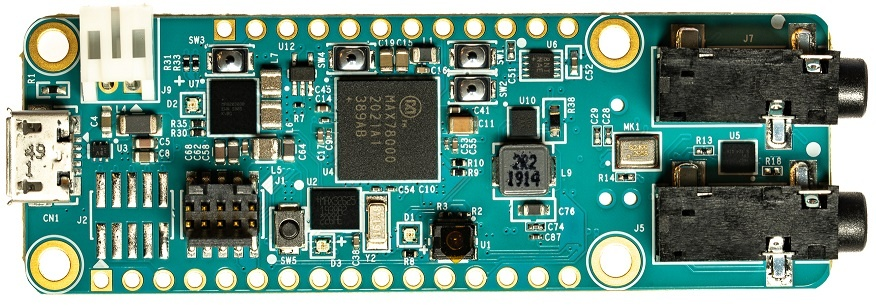
\psfig{file=Images/max78000fthr.jpg,width=0.8\textwidth}}
\setcaptioncitation{https://www.maximintegrated.com/en/products/microcontrollers/MAX78000.html}
\caption{Max78000 FTHR board}
\label{max78000_board}
\end{figure}

\section{CNN Accelerator}
\label{sec:456}
\quad The CNN accelerator consists of 64 parallel processors with 512KB of SRAM-based storage. Each processor includes a pooling unit and a convolutional engine with dedicated weight memory. Four processors share one data memory. These are further organized into groups of 16 processors that share common controls. A group of 16 processors operates as a slave to another group or independently. Data is read from SRAM associated with each processor and written to any data memory located within the accelerator. Any given processor has visibility of its dedicated weight memory and the Data memory instance it shares with the three others.
The CNN accelerator has multiple processors and it was fundamental to understand its functioning and its weights distribution in order to be able to implement a CL model.

%\begin{figure}[!ht]
%\centerline{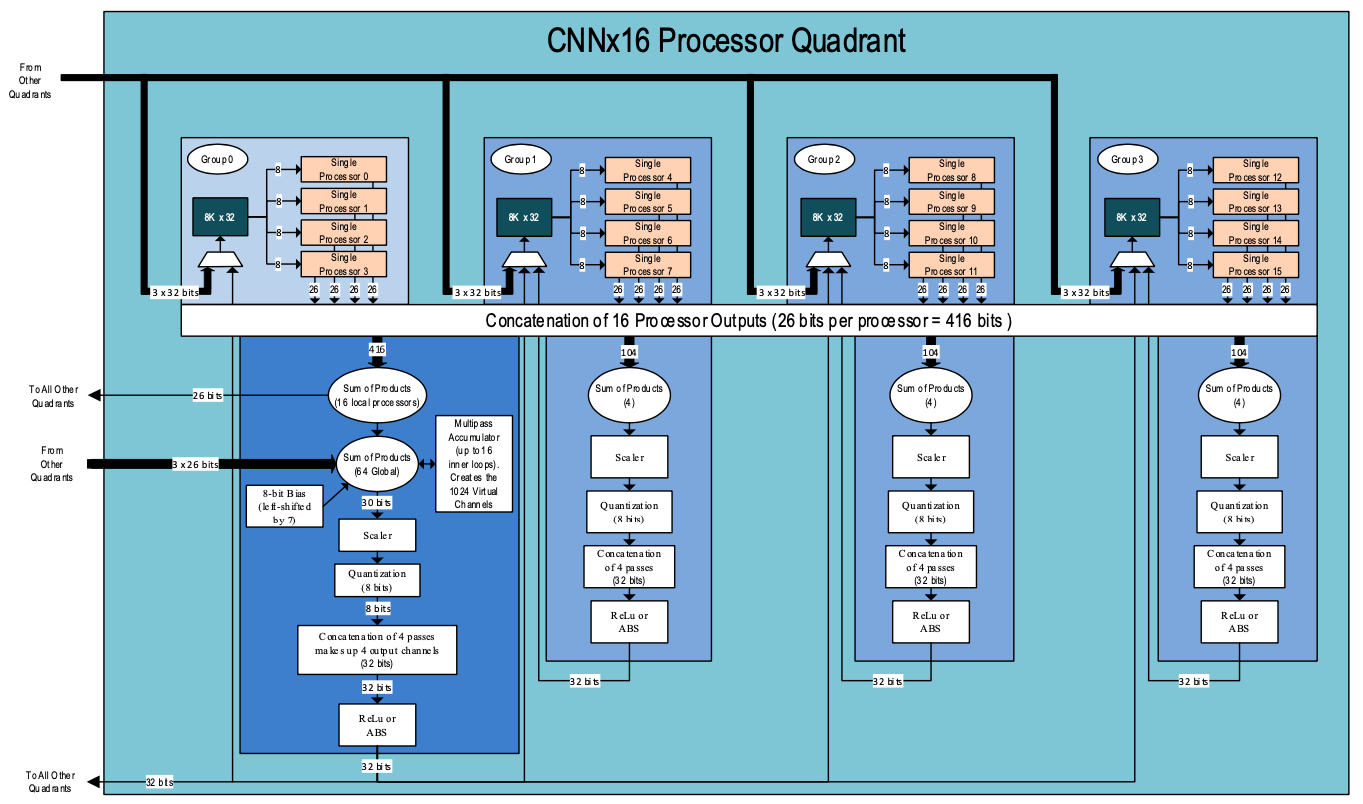
\psfig{file=CNN_accelerator_structure.png,width=0.%9\textwidth}}
%\caption{A quadrant of a CNN accelerator structure}
%\label{cnn_accelerator_structure}
%\end{figure}

\section{CNN model}
\label{sec:457}
\quad The CNN model used in this paper is a five-layer model composed of four convolutional layers with MaxPool and AvgPool and a last linear layer, followed by a Softmax function that extract the percentage of each class. 
The first layer gets an input matrix of 28x28x1, which is an image from Mnist dataset or Emnist dataset. Following, the matrix is convoluted and pooled to obtain a smaller one used to compute the next steps. 
In the end, there is the only one layer that uses biases, all of which are added at each output of the last neurons. 
Each layer uses an activation function named ReLU function, seen in figure \ref{relu}. This function is necessary to map every number into zero if less than zero or from 0 to 127 if greater than zero.

\begin{figure}[!ht]
\centerline{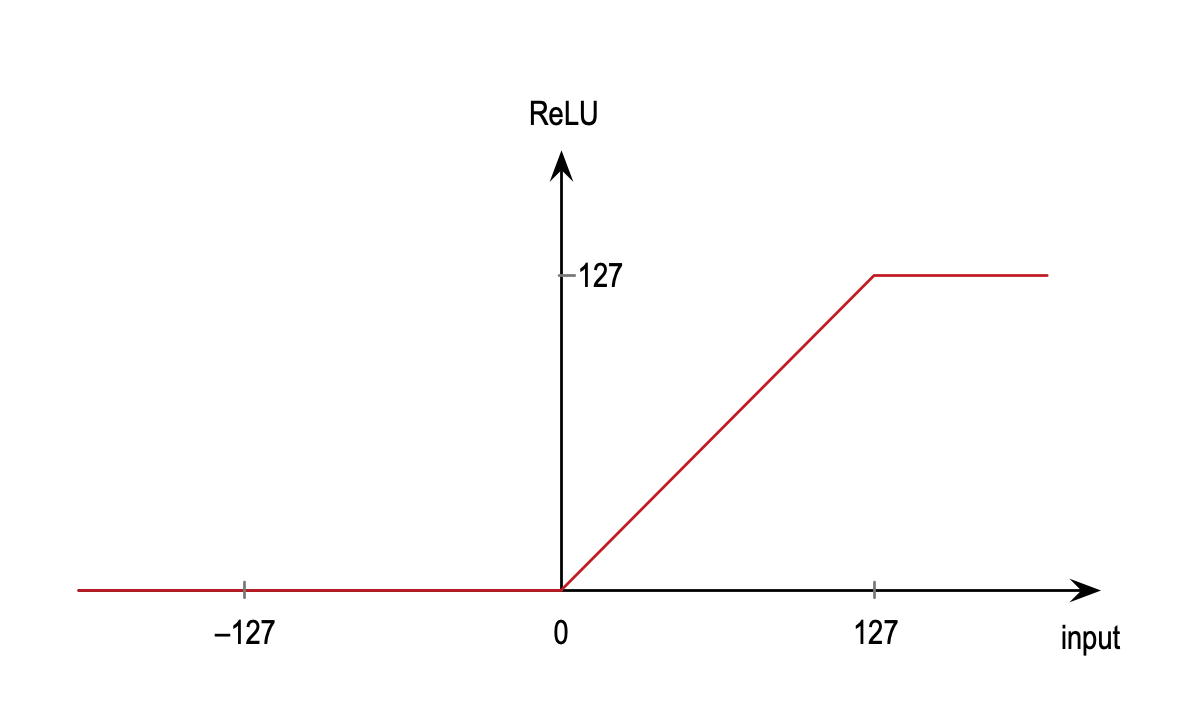
\psfig{file=Images/relu.png,width=0.6\textwidth}}
\setcaptioncitation{https://github.com/MaximIntegratedAI/ai8x-synthesis/blob/develop/docs/relu.png}
\caption{Max78000 relu function}
\label{relu}
\end{figure}

\clearpage
\newpage
\mbox{~}
\clearpage
\newpage